\documentclass[tikz]{standalone}
\usetikzlibrary{automata,positioning}
\begin{document}

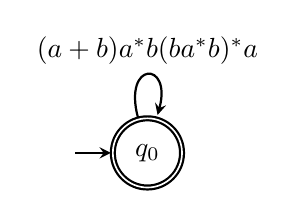
\begin{tikzpicture}[>=stealth,node distance=3cm,on grid,auto, thick, initial text=] 
  \node[state,initial,accepting] (q_0)   {$q_0$};

  \path[->]     (q_0) edge [loop above] node {$(a+b)a^*b(ba^*b)^*a$} (q_0);
  
                             
\end{tikzpicture}
\end{document}